\documentclass{tufte-book}
\usepackage[french]{babel}
\usepackage[utf8]{inputenc}

\hypersetup{colorlinks}% uncomment this line if you prefer colored hyperlinks (e.g., for onscreen viewing)

%%
% Book metadata
\title{Vim - Le guide pour les êtres humains\thanks{Merci à la communauté Vim.}}
\author[Vincent Jousse]{Vincent\ Jousse}
\publisher{Vincent Jousse}

%%
% If they're installed, use Bergamo and Chantilly from www.fontsite.com.
% They're clones of Bembo and Gill Sans, respectively.
%\IfFileExists{bergamo.sty}{\usepackage[osf]{bergamo}}{}% Bembo
%\IfFileExists{chantill.sty}{\usepackage{chantill}}{}% Gill Sans

%\usepackage{microtype}

%%
% Just some sample text
\usepackage{lipsum}

%%
% For nicely typeset tabular material
\usepackage{booktabs}

%%
% For graphics / images
\usepackage{graphicx}
\setkeys{Gin}{width=\linewidth,totalheight=\textheight,keepaspectratio}
\graphicspath{{graphics/}}

% The fancyvrb package lets us customize the formatting of verbatim
% environments.  We use a slightly smaller font.
\usepackage{fancyvrb}
\fvset{fontsize=\normalsize}

%%
% Prints argument within hanging parentheses (i.e., parentheses that take
% up no horizontal space).  Useful in tabular environments.
\newcommand{\hangp}[1]{\makebox[0pt][r]{(}#1\makebox[0pt][l]{)}}

%%
% Prints an asterisk that takes up no horizontal space.
% Useful in tabular environments.
\newcommand{\hangstar}{\makebox[0pt][l]{*}}

%%
% Prints a trailing space in a smart way.
\usepackage{xspace}

% Format code using pygment
\usepackage{minted}
\usemintedstyle{solarized}
%\definecolor{bg}{RGB}{0,43,54}
%Light bg
\definecolor{bg}{RGB}{253,246,227}

%%
% Some shortcuts for Tufte's book titles.  The lowercase commands will
% produce the initials of the book title in italics.  The all-caps commands
% will print out the full title of the book in italics.
\newcommand{\vdqi}{\textit{VDQI}\xspace}
\newcommand{\ei}{\textit{EI}\xspace}
\newcommand{\ve}{\textit{VE}\xspace}
\newcommand{\be}{\textit{BE}\xspace}
\newcommand{\VDQI}{\textit{The Visual Display of Quantitative Information}\xspace}
\newcommand{\EI}{\textit{Envisioning Information}\xspace}
\newcommand{\VE}{\textit{Visual Explanations}\xspace}
\newcommand{\BE}{\textit{Beautiful Evidence}\xspace}

\newcommand{\TL}{Tufte-\LaTeX\xspace}

% Prints the month name (e.g., January) and the year (e.g., 2008)
\newcommand{\monthyear}{%
  \ifcase\month\or January\or February\or March\or April\or May\or June\or
  July\or August\or September\or October\or November\or
  December\fi\space\number\year
}

% Prints an epigraph and speaker in sans serif, all-caps type.
\newcommand{\openepigraph}[2]{%
  %\sffamily\fontsize{14}{16}\selectfont
  \begin{fullwidth}
  \sffamily\large
  \begin{doublespace}
  \noindent\allcaps{#1}\\% epigraph
  \noindent\allcaps{#2}% author
  \end{doublespace}
  \end{fullwidth}
}

% Inserts a blank page
\newcommand{\blankpage}{\newpage\hbox{}\thispagestyle{empty}\newpage}

\usepackage{units}

% Typesets the font size, leading, and measure in the form of 10/12x26 pc.
\newcommand{\measure}[3]{#1/#2$\times$\unit[#3]{pc}}

% Macros for typesetting the documentation
\newcommand{\hlred}[1]{\textcolor{Maroon}{#1}}% prints in red
\newcommand{\hangleft}[1]{\makebox[0pt][r]{#1}}
\newcommand{\hairsp}{\hspace{1pt}}% hair space
\newcommand{\hquad}{\hskip0.5em\relax}% half quad space
\newcommand{\TODO}{\textcolor{red}{\bf TODO!}\xspace}
\newcommand{\ie}{\textit{i.\hairsp{}e.}\xspace}
\newcommand{\eg}{\textit{e.\hairsp{}g.}\xspace}
\newcommand{\na}{\quad--}% used in tables for N/A cells
\providecommand{\XeLaTeX}{X\lower.5ex\hbox{\kern-0.15em\reflectbox{E}}\kern-0.1em\LaTeX}
\newcommand{\tXeLaTeX}{\XeLaTeX\index{XeLaTeX@\protect\XeLaTeX}}
% \index{\texttt{\textbackslash xyz}@\hangleft{\texttt{\textbackslash}}\texttt{xyz}}
\newcommand{\tuftebs}{\symbol{'134}}% a backslash in tt type in OT1/T1
\newcommand{\doccmdnoindex}[2][]{\texttt{\tuftebs#2}}% command name -- adds backslash automatically (and doesn't add cmd to the index)
\newcommand{\doccmddef}[2][]{%
  \hlred{\texttt{\tuftebs#2}}\label{cmd:#2}%
  \ifthenelse{\isempty{#1}}%
    {% add the command to the index
      \index{#2 command@\protect\hangleft{\texttt{\tuftebs}}\texttt{#2}}% command name
    }%
    {% add the command and package to the index
      \index{#2 command@\protect\hangleft{\texttt{\tuftebs}}\texttt{#2} (\texttt{#1} package)}% command name
      \index{#1 package@\texttt{#1} package}\index{packages!#1@\texttt{#1}}% package name
    }%
}% command name -- adds backslash automatically
\newcommand{\doccmd}[2][]{%
  \texttt{\tuftebs#2}%
  \ifthenelse{\isempty{#1}}%
    {% add the command to the index
      \index{#2 command@\protect\hangleft{\texttt{\tuftebs}}\texttt{#2}}% command name
    }%
    {% add the command and package to the index
      \index{#2 command@\protect\hangleft{\texttt{\tuftebs}}\texttt{#2} (\texttt{#1} package)}% command name
      \index{#1 package@\texttt{#1} package}\index{packages!#1@\texttt{#1}}% package name
    }%
}% command name -- adds backslash automatically
\newcommand{\docopt}[1]{\ensuremath{\langle}\textrm{\textit{#1}}\ensuremath{\rangle}}% optional command argument
\newcommand{\docarg}[1]{\textrm{\textit{#1}}}% (required) command argument
\newenvironment{docspec}{\begin{quotation}\ttfamily\parskip0pt\parindent0pt\ignorespaces}{\end{quotation}}% command specification environment
\newcommand{\docenv}[1]{\texttt{#1}\index{#1 environment@\texttt{#1} environment}\index{environments!#1@\texttt{#1}}}% environment name
\newcommand{\docenvdef}[1]{\hlred{\texttt{#1}}\label{env:#1}\index{#1 environment@\texttt{#1} environment}\index{environments!#1@\texttt{#1}}}% environment name
\newcommand{\docpkg}[1]{\texttt{#1}\index{#1 package@\texttt{#1} package}\index{packages!#1@\texttt{#1}}}% package name
\newcommand{\doccls}[1]{\texttt{#1}}% document class name
\newcommand{\docclsopt}[1]{\texttt{#1}\index{#1 class option@\texttt{#1} class option}\index{class options!#1@\texttt{#1}}}% document class option name
\newcommand{\docclsoptdef}[1]{\hlred{\texttt{#1}}\label{clsopt:#1}\index{#1 class option@\texttt{#1} class option}\index{class options!#1@\texttt{#1}}}% document class option name defined
\newcommand{\docmsg}[2]{\bigskip\begin{fullwidth}\noindent\ttfamily#1\end{fullwidth}\medskip\par\noindent#2}
\newcommand{\docfilehook}[2]{\texttt{#1}\index{file hooks!#2}\index{#1@\texttt{#1}}}
\newcommand{\doccounter}[1]{\texttt{#1}\index{#1 counter@\texttt{#1} counter}}

% Keys shortcuts
\newcommand{\tesc}{\hlred{Esc} (\hlred{Échap})\xspace}
\newcommand{\ttesc}{la touche \tesc}
\newcommand{\tshift}{\hlred{Shift}\xspace}
\newcommand{\ttshift}{la touche \tshift}
\newcommand{\ti}{\hlred{i}\xspace}
\newcommand{\tti}{la touche \ti}
\newcommand{\ttm}{la touche \hlred{m}\xspace}
\newcommand{\tto}{la touche \hlred{o}\xspace}
\newcommand{\tp}{\hlred{p}\xspace}
\newcommand{\ttp}{la touche \tp}
\newcommand{\tv}{\hlred{v}\xspace}
\newcommand{\ttv}{la touche \tv}
\newcommand{\ty}{\hlred{y}\xspace}
\newcommand{\tty}{la touche \ty}

\newcommand{\vimscmd}[1]{\fcolorbox{black}{bg}{\hlred{\Verb|{\footnotesize #1}|}}}
\newcommand{\vimcmd}[1]{\fcolorbox{black}{bg}{\hlred{\Verb|#1|}}}

\newcommand{\scmd}[1]{\fcolorbox{black}{white}{\hlred{\Verb|{\footnotesize #1}|}}}
\newcommand{\ncmd}[1]{\fcolorbox{black}{white}{\hlred{\Verb|#1|}}}

\newcommand{\vim}{\emph{Vim}\xspace}
\newcommand{\vimrc}{\emph{.vimrc}\xspace}


% Generates the index
\usepackage{makeidx}
\makeindex


\begin{document}

% Front matter
\frontmatter

% r.1 blank page
\blankpage

% r.3 full title page
\maketitle


% v.4 copyright page
\newpage
\begin{fullwidth}
~\vfill
\thispagestyle{empty}
\setlength{\parindent}{0pt}
\setlength{\parskip}{\baselineskip}
Copyright \copyright\ \the\year\ \thanklessauthor

\par\smallcaps{Publié par \thanklesspublisher}

\par\smallcaps{Style \LaTeX{} \url{http://tufte-latex.googlecode.com}}

\par Si vous n'avez pas payé cette copie, bah tant pis pour moi ;) Mais sachez que vous auriez dû !

\end{fullwidth}

% r.5 contents
\tableofcontents

\listoffigures

\listoftables

% r.7 dedication
\cleardoublepage
~\vfill
\begin{doublespace}
\noindent\fontsize{18}{22}\selectfont\itshape
\nohyphenation
Merci à ma femme et mes enfants qui ont permis à ce livre de voir le jour.
\end{doublespace}
\vfill
\vfill

% r.9 introduction
\cleardoublepage

\chapter*{Introduction}

\newthought{Lorsque le besoin} d'écrire ou de coder se fait se sentir, le choix d'un éditeur de texte est primordial. Il en existe énormément sur le "marché", mais peu d'entre eux peuvent se targuer d'environ 40 ans d'existence. C'est le cas d'\emph{Emacs} (\url{http://www.gnu.org/software/emacs/}), de \emph{Vi} et de son "successeur amélioré" \vim (\url{http://www.vim.org/}). Ils ont été créés dans les années 70 et sont toujours très utilisés actuellement. Comme vous avez sans doute pu le voir, ce n'est pas grâce à la beauté de leur site internet ou à l'efficacité de leur communication. Voici quelques \textbf{raisons de leur succès} :

\begin{description}
    \item[Pour la vie] \hfill \\ Ils s'apprennent une fois et s'utilisent pour toujours. Dans un monde où les technologies/langages changent tout le temps, c'est une aubaine de pouvoir investir sur du long terme.
    \item[Partout] \hfill \\ Ils sont disponibles sur toutes les plateformes possibles et imaginables (et l'ont toujours été).
    \item[Augmentent votre vitesse d'édition de texte] \hfill \\ Grâce à leurs particularités (notamment l'utilisation du clavier), ils permettent d'éditer du texte très rapidement.
    \item[Couteaux suisses] \hfill \\ Ils permettent d'éditer tout et n'importe quoi. Quand vous changerez de langage de programmation, vous n'aurez pas à changer d'éditeur. À noter que ce livre a bien sûr été écrit avec \vim.
\end{description}

Et pourtant, ces éditeurs de texte restent difficiles à apprendre. Non pas qu'ils soient plus compliqués qu'autre chose, non pas que vous ne soyez pas à la hauteur, mais plutôt à cause d'un manque de pédagogie des différentes documentations.

Ce livre a pour but de pallier ce manque en vous guidant tout au long de votre découverte de \vim\sidenote{Je laisse \emph{Emacs} à ceux qui savent. Pour un bref comparatif c'est ici : \url{http://fr.wikipedia.org/wiki/Guerre_d'\%C3\%A9diteurs}. Les goûts et les couleurs …}. Il ne prétend pas être un guide exhaustif, vous pouvez essayer \emph{A Byte of \vim} pour celà : \url{http://www.swaroopch.org/notes/Vim}. En revanche, il prétend diminuer la marche à franchir pour s'habituer à \vim. À mon sens, le plus compliqué avec \vim, c'est de ne pas se décourager de suite et de trouver une méthode qui vous permette de l'apprendre au fur et à mesure. Nous avons tous un travail à effectuer au quotidien, et perdre toute sa productivité à cause d'un changement d'éditeur de texte n'est pas envisageable.

Vous trouverez beaucoup de personnes pour vous dire \og mais tu n'as qu'à t'y mettre pour de bon \fg, \og tu verras après ça va aller mieux \fg, certes, mais vous devez toujours être productif au jour le jour, ça ne change rien au problème. L'approche de ce livre est la suivante :

\begin{enumerate}
    \item Disposer d'un \vim un temps soit peu moderne : coloration syntaxique et jolies couleurs.
    \item Pouvoir utiliser \vim comme n'importe quel autre éditeur de texte : éditer facilement du code et naviguer entre les fichiers en utilisant la souris.
    \item Apprendre des raccourcis clavier et se passer de la souris au fur et à mesure.
    \item Installer un \emph{best-of} des plugins pour commencer à tirer partie de la puissance de \vim.
\end{enumerate}

À partir du point numéro 2, vous pourrez déjà utiliser \vim au quotidien sans perdre énormément de productivité. Et c'est là que la différence se fait : si vous pouvez intégrer \vim dans votre quotidien c'est gagné. Vous aurez ensuite toute votre vie pour connaître tous les raccourcis clavier.

Vous aussi vous en avez marre d'attendre la release de TextMate 2\footnote{À noter que depuis l'écriture de ce livre, le code de TextMate 2 a été publié sous licence GPL : \url{https://github.com/textmate/textmate}} ? D'essayer le n-ième éditeur à la mode et de devoir tout réapprendre et ce jusqu'à la prochaine mode ? De devoir changer d'éditeur quand vous passez de votre Mac, à votre Windows, à votre Linux ? Alors vous aussi, rejoignez la communauté des gens heureux de leur éditeur de texte. \textbf{Le changement, c'est maintenant} !

\section{Pour qui ?}

\newthought{Toute personne} étant amenée à produire du texte (code, livre, rapports, présentations, ...) de manière régulière. Les développeurs sont bien sûr une cible privilégiée, mais pas uniquement.

Par exemple vous êtes :
\begin{description}
    \item[Étudiant] Si vous voulez faire bien sur un CV, c'est un must (en plus d'être un attrape geekette en puissance\footnote{À confirmer.}). Vous aurez un outil unique pour écrire tout ce que vous avez à écrire (et que vous pourrez réutiliser tout au long de votre carrière) : vos rapports en \LaTeX, vos présentations\footnote{En utilisant \emph{impress.js} par exemple : \url{http://bartaz.github.com/impress.js}. Basé sur du HTML/JS/CSS, je vous le recommande grandement pour des présentations originales et basées sur des technologies non propriétaires.}, votre code (si vous avez besoin d'OpenOffice ou de Word pour écrire vos rapports, il est temps de changer d'outil et d'utiliser \LaTeX).
    \item[Enseignant] Il est temps de montrer l'exemple et d'apprendre à vos étudiants à bien utiliser un des outils qui leur servira à vie, bien plus qu'un quelconque langage de programmation.
    \item[Codeur] Investir dans votre outil de tous les jours est indispensable. Quitte à apprendre des raccourcis claviers, autant le faire de manière utile. Si cet investissement est encore rentable dans 10 ans, c'est ce que l'on pourrait appeler l'investissement parfait, c'est \vim.
    \item[Administrateur système Unix] Si vous utilisez \emph{Emacs} vous êtes pardonnable. Si vous utilisez nano/pico je ne peux plus rien pour vous, sinon il est grand temps de s'y mettre les gars. Administrer un système Unix à distance est un des cas d'utilisation parfait pour \vim (un éditeur de texte surpuissant ne nécessitant pas d'interface graphique).
    \item[Écrivain] Si vous écrivez en markdown/reStructuredText/WikiMarkup ou en \LaTeX, \vim vous fera gagner beaucoup de temps. Vous ne pourrez plus repasser à un autre éditeur, ou vous voudrez le "Vimifier" à tout prix.
\end{description}

Faites moi confiance, je suis passé et repassé par ces 5 rôles, mon meilleur investissement a toujours été \vim, et de loin.

\section{Ce que vous apprendrez (entre autres choses)}

\begin{itemize}
    \item Comment utiliser \vim comme un éditeur \og normal \fg{} d'abord (vous savez, ceux qui permettent d'ouvrir des fichiers, de cliquer avec la souris, qui ont une coloration syntaxique ...). En somme, la démystification de \vim qui vous permettra d'aller plus loin.
    \item Comment passer de l'édition de texte classique à la puissance de \vim, petit à petit (c'est là que l'addiction commence).
    \item Comment vous passer de la souris et pourquoi c'est la meilleure chose qu'il puisse vous arriver quand vous programmez/tapez du texte.
    \item Comment vous pouvez facilement déduire les raccourcis claviers avec quelques règles simples.
\end{itemize}

Si je devais le résumer en une phrase : puisque vous vous considérez comme {\bf un artiste, passez du temps à apprendre} comment utiliser l'outil qui vous permet de vous exprimer, une bonne fois pour toute.

\section{Ce que vous n'apprendrez pas (entre autres choses)}

\begin{itemize}
    \item Vous n'apprendrez pas comment installer/configurer \vim pour Windows. Pas que ce ne soit pas faisable, mais je n'ai que très peu de connaissances de Windows. Ça viendra peut-être, mais pas tout de suite. On couvrira ici Linux/Unix (et par extension Mac OS X).
    \item Vous n'apprendrez pas comment utiliser \emph{Vi} (notez l'absence du "m"). Je vais vous apprendre à être productif pour coder/produire du texte avec \vim, pas à faire le beau devant les copains avec \emph{Vi}\footnote{\vim est suffisant pour cela de toute façon.}. Pour ceux qui ne suivent pas, \emph{Vi} est "l'ancêtre de \vim (qui veut dire \emph{Vi} - \emph{IMproved}, \emph{Vi} amélioré)" et est installé par défaut sur tous les Unix (même sur votre Mac OS X).
    \item Vous n'apprendrez pas à connaitre les entrailles de \vim par c\oe ur : ce n'est pas une référence, mais un guide utile et pragmatique.
    \item Vous n'apprendrez pas comment modifier votre \vim parce que vous préférez le rouge au bleu : je vous ferai utiliser le thème \emph{Solarized} (\url{http://ethanschoonover.com/solarized}), il est parfait pour travailler.
\end{itemize}

\section{Le plus dur, c'est de commencer}

Alors, prêt pour l'aventure ? Prêt à sacrifier une heure pour débuter avec \vim, une semaine pour devenir familier avec la bête, et le reste de votre vie pour vous féliciter de votre choix ? Alors c'est parti ! Enfin presque, il faut qu'on parle avant.

\vim fait partie de ces outils avec lesquels vous allez galérer au début. Le but de ce guide est de vous mettre le pied à l'étrier et de diminuer la hauteur de la marche à franchir. Mais soyez conscients que vous mettre à \vim va vous demander de la volonté et quelques efforts. Comme on dit souvent, on n'a rien sans rien. Voici la méthode que je vous recommande pour apprivoiser la bête :

\begin{itemize}
    \item Essayez de faire entrer \vim dans vos habitudes. Suivez le premier chapitre de ce guide jusqu'à la partie concernant l'explorateur de fichiers utilisable à la souris \emph{The NERD Tree}. Ensuite, vous pourrez utiliser \vim comme un Notepad++ ou un TextMate ou un Sublime Text. Vous n'utiliserez que 1\% des capacités de \vim mais peu importe. Ce qui est important, c'est de le faire entrer dans votre quotidien.
    \item Gardez une feuille avec les principaux raccourcis imprimée à côté de vous. Le but ce n'est pas de les apprendre par cœur, mais c'est de les avoir à portée de main quand vous vous demanderez \og mais il y a certainement une façon plus efficace de faire cela \fg.
    \item Gardez la foi. Au début vous resterez un sceptique quant à l'utilité de tout réapprendre avec \vim. Et puis un jour vous aurez un déclic et vous vous demanderez pourquoi tous vos logiciels ne peuvent pas se contrôler avec les commandes de \vim.
    \item Gardez à l'esprit que c'est un investissement pour vos 20 prochaines années, et c'est bien connu, un investissement ce n'est pas complètement rentable de suite.
\end{itemize}

\bigskip

Trêve de bavardage, passons aux choses sérieuses. Go go go !

\mainmatter

\chapter{Rendre ViM utilisable}

Ça peut paraître étonnant comme approche, mais c'est pour moi la première chose à faire : rendre \emph{Vim} utilisable par un humain lambda. Si tout le monde semble s'accorder sur le fait que \emph{Vim} est un \textbf{éditeur très puissant}, tout le monde pourra aussi s'accorder sur le fait que de base, il est juste \textbf{imbitable}. Soyons honnête, sans une configuration par défaut minimale, utiliser \emph{Vim} est \textbf{contre-productif}. C'est à mon avis le premier obstacle à surmonter avant toute autre chose. C'est ce que les autres éditeurs ``Mainstream'' comme Textmate, Sublimetext, Notepad++ ou Netbeans proposent, c'est à dire un environnement à minima utilisable tel quel, même si l'on en n'exploite pas la totalité.

Voici donc ce qui manque à un \emph{Vim} nu (et ce qui est pour moi une \textbf{cause d'abandon pour beaucoup} d'entre vous) :

\begin{marginfigure}%
  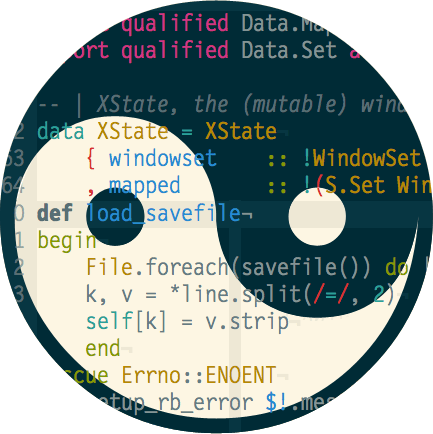
\includegraphics[width=\linewidth]{solarized-yinyang.png}
  \caption{Le thème Solarized en sombre et en clair.}
  \label{fig:solarized}
\end{marginfigure}

\begin{description}
    \item[Configuration par défaut] \emph{Vim} est configurable grâce à un fichier nommé \emph{vimrc}, qui est bien sur par défaut vide. La première étape va être d'avoir un fichier \emph{vimrc} par défaut.
    \item[Coloration syntaxique] De base, \emph{Vim} est tout blanc et tout moche. On va utiliser par défaut le thème Solarized (\url{http://ethanschoonover.com/solarized}). Si votre but est d'être efficace (et pas de préférer le rose au bleu), c'est le meilleur thème disponible actuellement (tout éditeur de texte confondu). La figure \ref{fig:solarized} vous donne une idée des deux look disponibles (clair ou sombre). Pour ma part j'utilise le thème sombre.
    \item[Explorateur de fichiers] Si vous utilisez \emph{Vim} avec une interface graphique (ce qui est le cas de 99\% d'entre vous je suppose) vous avez par défaut un menu ``Fichier'' vous permettant d'ouvrir un fichier. C'est certes un bon début, mais avoir à disposition un explorateur de projet à la Netbeans ou à la Textmate peut s'avérer très pratique. Pour obtenir le même comportement, nous utiliserons Nerdtree.
\end{description}

Ce chapitre est indispensable si vous n'avez que peu de connaissances Vimesques pour l'instant. À la fin de ce chapitre, vous aurez un \emph{Vim} dont vous pourrez commencer à vous servir pour vos tâches de tous les jours.

\printindex

\end{document}
